\section{Two-dimensional disks with beta cooling}\label{result_2d}
We begin in the 2D limit with standard beta cooling  to facilitate comparison 
with previous studies. The disk
material is assumed to be confined to the midplane, and $\delta v_z=0$. 
We make the replacement  
$\rho \to \Sigma$, re-interpret $P$ as the vertically-integrated
pressure, and set $\Gamma=1$. % without loss of generality. 
%big gamma only controls vertical structure
%can absorb big gamma into def of cs
The gravitational potential perturbation remains 3D and its midplane
value is given by    
\begin{align}
  \delta \Phi(z=0) = -\frac{2 \pi G}{|k|}\delta\Sigma
\end{align}
\citep{shu70}.
 
The linearized equations yield an algebraic dispersion relation $s =
s(k)$. We write this  
in terms of the dimensionless growth rate $S = s/\Omega$ and
wavenumber $K=kH = k c_{s0}/\Omega$ as
\begin{align}\label{thindisk}
  f(S,K)\equiv AD - BC = 0,   
\end{align}
where the functions $A,B,C,D$ are given in Appendix \ref{2ddisp}. % Note
% that these functions, as given, do not assume any $\alpha$-$\beta$
% relation.
We use this generalized dispersion relation  to investigate GI driven 
by cooling in \S\ref{2d_inviscid}; and GI driven by viscosity 
in \S\ref{2dvisc}. 




\subsection{Inviscid limit}\label{2d_inviscid}
We first simplify the problem by setting $\alpha = \alpha_b = 0$. This
eliminates viscous heating and forces, allowing us to quantify the 
\emph{sole} effect of cooling on the 
perturbations. %KMK
We emphasize that destabilization is independent of the effect of decreasing temperature on the instantaneous
value of the classic-$Q$. A time-independent heat source should be
invoked to balance the imposed cooling to allow an equilibrium to be
defined ($\mathcal{H}_\mathrm{ext}\neq 0$). Alternatively, we are
assuming viscosity only provides a background heating and does not
play an active role in the perturbed state. %may or may not be true in a real
                                %disk because we are using viscosity
                                %as proxy for turbulence
                                %maybe turb heating actually behaves
                                %like background heat source only 
	%KMK interesting points. discuss later?
Eq. \ref{thindisk} becomes 
\begin{align}\label{inviscid}
%  &\beta S^3 + S^2 - \beta \left\{ \frac{2|K|}{\qtwo} - \left[2(2-q) +
%    \gamma K^2\right]\right\}S \notag\\ &- \left[\frac{2|K|}{\qtwo} - 2(2-q)\right]
%  = 0. 
  S^2 = \frac{2|K|}{Q} - 2(2-q) - \left(\frac{\theta + \beta \gamma
    S}{1+\beta S}\right)K^2, 
\end{align}
similar to the classic dispersion relation
(Eq. \ref{classic_dr}), which may be obtained by taking the limit
$|\beta S|\to\infty$. %then setting gamma=1. other params fixed
                      %(finite theta)
The first term on the right-hand-side represents destabilization by self-gravity; 
the second and third terms represent stabilization by rotation and
pressure, respectively. The imposed cooling/irradiation only affects the
pressure response. %KMK no...? {\bf do we need to explain the terms again?}

Eq. \ref{inviscid} is a cubic equation in $S$. The 
Routh-Hurwitz criteria imply that stability is ensured if 
\begin{align}\label{stable_condition}
  \gamma > \theta \quad \text{and} \quad 
  Q > \frac{1}{\sqrt{2\theta(2-q)}} 
\end{align}
are both satisfied. 
%gamma/theta condition is related to some kind of thermal instability
%oscilitory convection?? 
%second condition concerning Q is associated with self-g 
A third criterion, $2(2-q)\gamma Q^2>1$, is formally required, but this
is implied by Eq. \ref{stable_condition}. 
Notice these conditions do not actually depend on the cooling time. 
At fixed $Q$, the second stability condition eventually fails for
decreasing $\theta$, i.e. if perturbations are allowed
to cool to sufficiently low temperatures.  

%{\bf KMK maybe more words here about apparent trend of $Q \rightarrow \inf$ for small $\theta$
%even forward ref. lengthscales below?}

If only real growth rates are considered, then violating the second
condition in Eq. \ref{stable_condition} alone is sufficient for instability. 
%from property of cubic crossing the real axis 
In that case the wavenumbers satisfying
\begin{align}
  \theta K^2 - \frac{2}{Q}|K| + 2(2-q) < 0 
\end{align}
are unstable. The range of unstable wavenumbers
increases with decreasing irradiation $\theta$. For $\theta\ll 1$ this range is 
$(2-q)Q\lesssim|K|\lesssim2/\theta Q$. Without irradiation there is no
upper limit to unstable wavenumbers, which could have implications for
numerical simulations probing large wavenumbers and small scales 
at high resolution (see \S\ref{prev_works}). 

Consider the most unstable wavenumber $|K_*|$ at which $\p S/\p|K| =
0$ and $S = S_*$. By differentiating Eq. \ref{inviscid}, we obtain 
\begin{align}\label{kstar}
%  |K_*| = \frac{1}{\gamma \qtwo} \left(1 + \frac{1}{\beta S_*}\right). 
  |K_*| = \frac{1+\beta S_*}{Q\left(\theta + \gamma \beta S_*\right)}
\end{align}
%Eq. \ref{kstar} describes how the most unstable  mode is affected by
%cooling ($\beta$) and external heating ($\theta$). 
Inserting this into Eq. \ref{inviscid}, we find the maximum growth
rate satisfies
\begin{align}\label{inviscid_max}
%  S_*^3 + \left[2(2-q)  - \frac{1}{\gamma \qtwo^2}\right]S_* - \frac{1}{\gamma
%    \qtwo^2 \beta} = 0.
  S_*^2 = \frac{1+\beta S_*}{Q^2\left(\theta + \beta\gamma S_*\right)}
  - 2(2-q).
\end{align}
Eq. \ref{kstar}---\ref{inviscid_max} imply $\p_\beta|K_*|,\,\p_\beta
S_*<0 $ for $\gamma>\theta$. Then as cooling becomes more rapid, the maximum 
growth rate increases, and the most unstable wavelength decreases. 
%show dK*/dbeta < 0 
%by diff K* wrt beta and diff S* wrt beta from the equations
%and elim dS*/d beta 
For $|S_*|\ll1$, Eq. \ref{inviscid_max} gives the simple solution 
\begin{align}
  \beta S_*\simeq \frac{1-2(2-q)Q^2\theta}{2(2-q)Q^2\gamma-1}.  
\end{align} 
%Assuming the denominator is positive definite (see below for the case
%when it vanishes),  
Thus $S_*\to0$ as $\beta\to\infty$, but growth rates are never zero
for any finite $\beta$. That is, the disk can be formally unstable for
arbitrarily long cooling times.     
 
Next, we consider two special cases: $\theta=0$, so perturbations are
cooled towards zero temperature \citep[typically employed in
numerical simulations, e.g.][]{gammie01}; and $\theta=1$, where the
equilibrium disk temperature equals the irradiation temperature.  




\begin{figure}
  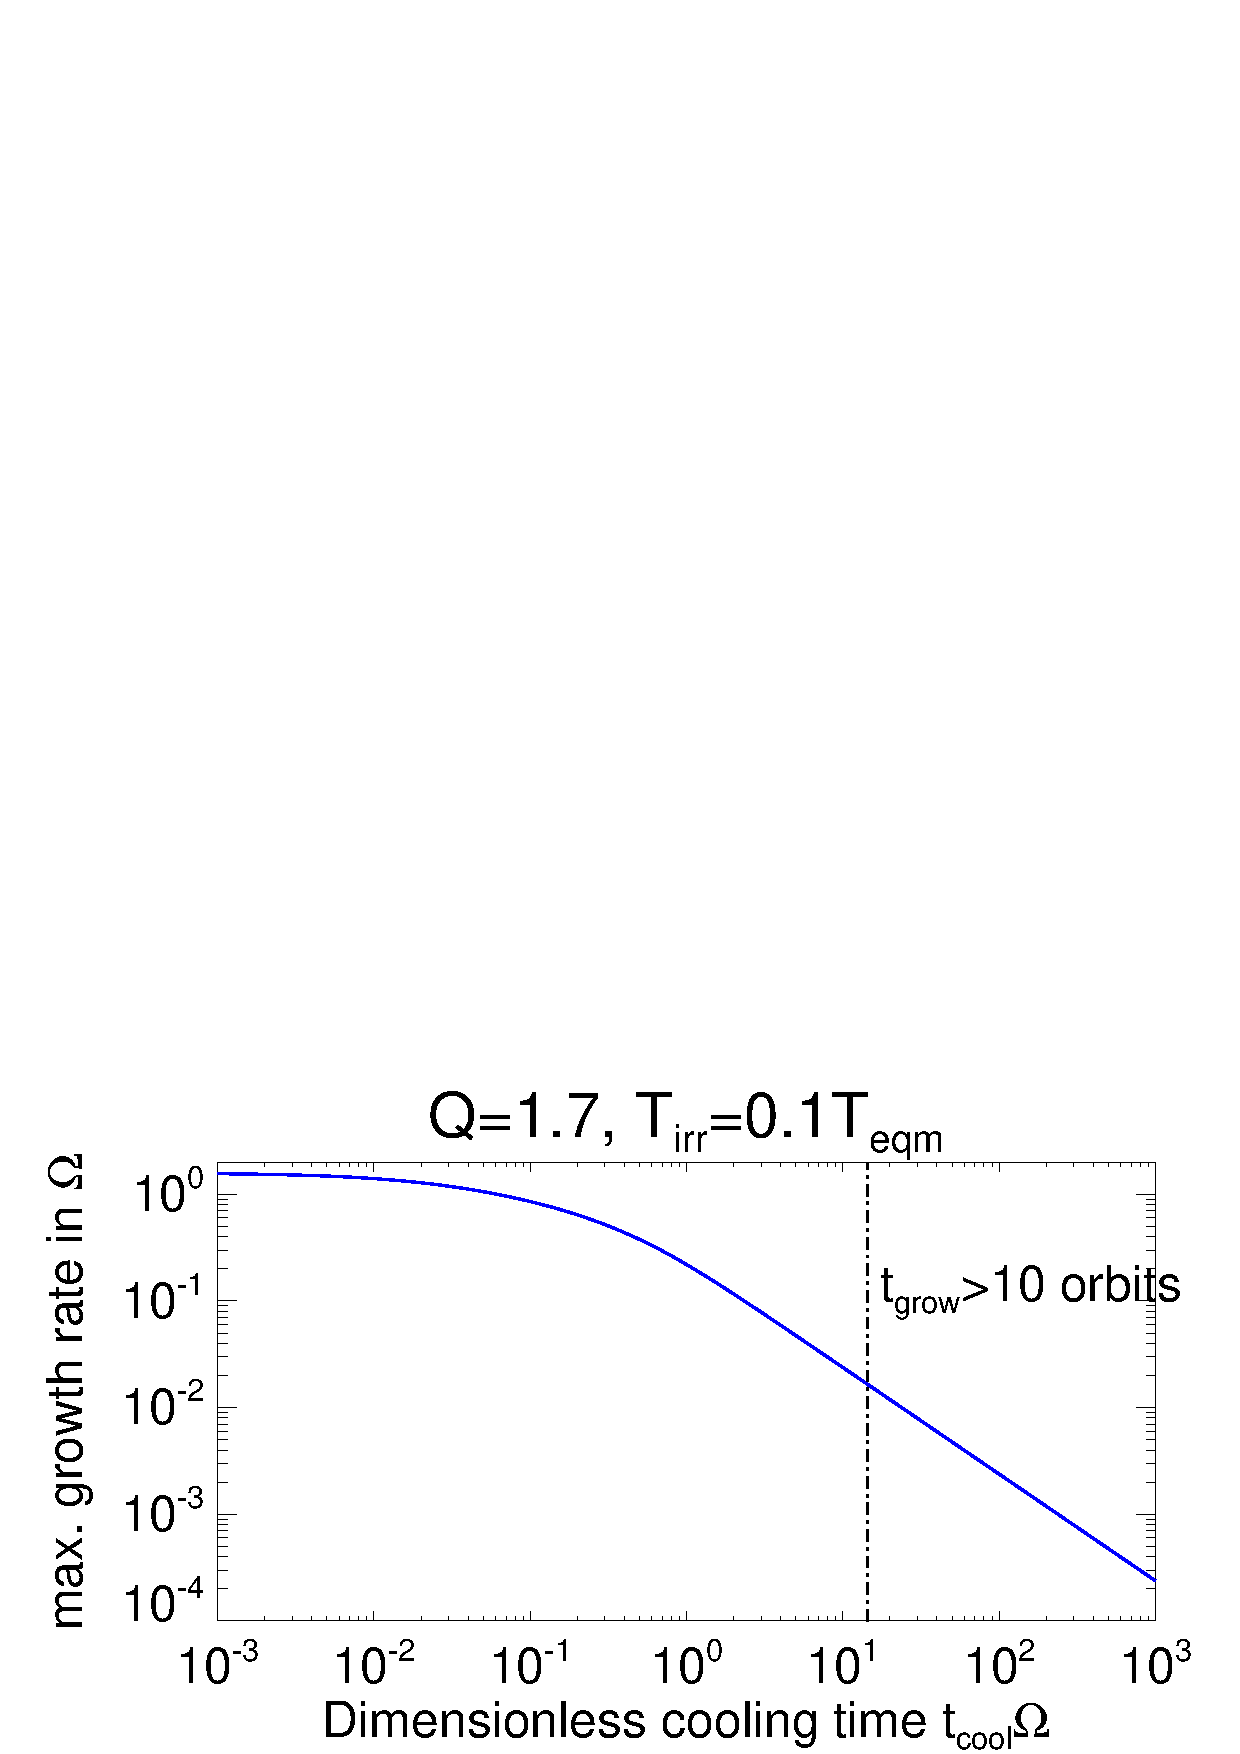
\includegraphics[width=\linewidth,clip=true,trim=0cm 0cm 0cm
    0.0cm]{figures/2dinvisc_theta}
  \caption{
    Growth rates for the 2D inviscid problem as a function of
    the cooling time $\beta$ for two irradiation levels: $\theta=0.1$ (black) and
    $\theta=0.33$ (orange). For each case the vertical dashed-dotted lines mark the cooling times beyond which
    growth rates are longer than 10 orbits. 
    \label{invisc_theta}}
\end{figure}










\subsubsection{$\theta = 0$}\label{theta0}
For $\beta$-cooling with $\theta=0$, the disk is unconditionally
unstable for finite $Q$, although instability occur on smaller scales
as $Q$ increases.  The $\beta\to0$ limit corresponds to a 
pressureless disk (not merely isothermal).   

%for definiteness 
Let us consider a disk with 
\begin{align}\label{qcrit_def}
  \qtwo = \frac{1}{\sqrt{2\gamma(2-q)}}\equiv Q_{\mathrm{crit}},
\end{align} 
%{\bf KMK $\gamma = \theta$ from eq. 47? I'm missing something}
which is the condition for marginal stability in an adiabatic disk. 
How does finite cooling destabilize the disk?  
Inserting Eq. \ref{qcrit_def} into Eq. \ref{inviscid_max} with 
$\theta=0$, we find 
\begin{align}\label{sstar}
  S_*^3 = \frac{1}{\gamma Q_\mathrm{crit}^2 \beta}. 
\end{align}
The maximum growth rate, $S_*\propto \beta^{-1/3}$, smoothly
increases with decreasing $\beta$. 
%Instability formally occurs for
%arbitrarily long but finite cooling times. 
%Instability does not require the
%cooling time to be below some critical value. 

We can define a characteristic cooling
time $\beta_*$ as that which removes pressure support against
self-gravity over the natural lengthscale in the problem, the
scale-height $H$. We thus set $|K_*|=1$ and find, for the Keplerian
disk,  

\begin{align}\label{betastar}
  \beta_* = \frac{1}{\left(\sqrt{\gamma} - 1\right)^{3/2}}. 
\end{align}
This equation gives remarkably similar values 
of the cooling times below which 
numerical simulations show dynamical disk fragmentation 
\citep{gammie01,rice05,rice11}. These simulations employ the same beta  
cooling prescription with $\theta=0$, and determine the fragmentation
boundary, $\beta_c$, as a function of the adiabatic index $\gamma$.  
Table \ref{bstar_compare} shows rough agreement between $\beta_*$ and 
$\beta_c$.  

\begin{deluxetable}{rrrr}
  \tablecolumns{4}
  \tablecaption{Characteristic cooling times as a function of
    $\gamma$. \label{bstar_compare}
  }
  \tablehead{
    %\colhead{}    &  \multicolumn{3}{c}{Non-shell Stars} &   \colhead{}   &
    %\multicolumn{3}{c}{Shell Stars} \\
    %\cline{2-4} \cline{6-8} \\
    \colhead{$\gamma$}   & \colhead{Eq. \ref{betastar}, $\beta_*$} &
    \colhead{Simulation, $\beta_c$} &  \colhead{Reference}
  }
\startdata
 $7/5$ & 12.75 & 12---13 & \cite{rice05}\\
$1.6$  &  7.33 & 8 & \cite{rice11}\\
$5/3$  &  6.37 & 6---7 & \cite{rice05}\\
$2$    &  3.75 & 3 & \cite{gammie01}
\enddata
\end{deluxetable}

\subsubsection{$\theta = 1$}\label{theta1}
Standard beta cooling with $\theta=1$ corresponds to 
`thermal relaxation': the temperature is restored to its initial
value over the cooling time \citep{lin15,mohandas15}. In this case no
additional heat source need be invoked to define an inviscid steady state. From
Eq. \ref{stable_condition}, the instability condition is $Q<1$. %no
                                %beta dependence
This is the same as the classic Toomre condition for an isothermal
disk (which may be obtained from Eq. \ref{inviscid}  by taking
$|\beta S|\to 0$). In this respect, a 
fully irradiated disk, in that the equilibrium temperature is set
externally, behaves isothermally regardless of the cooling time. 


%The most unstable wavenumber and growth
%rates vary weakly with $\beta$.  
% {\bf KMK: summarize boring result? not sure 
%what this simplifies to in comparison to other limits?}.

%nothing interesting here 



%\subsubsection{Expected maximum stress}
%{\bf for notes only} 
%A reasonable assumption is that in the non-linear regime 
%there is an associated turbulent viscosity that may be estimated  
%as $\nu \sim l^2s$, where the lengthscale $l\sim 1/k$; which
%translates to $\alpha\sim S/K^2$.  
%
%Using Eq. \ref{pressureless}, we find that 
%\begin{align}\label{max_alpha}
%  \mathrm{max}\left(\frac{S}{K^2}\right) = \frac{3^{3/2}}{2^{7/2}\left(2-q\right)^{3/2}Q^2}
%\end{align}
%in the limit $\beta\to 0$. This maximum is occurs at wavenumber $|K| =
%4Q(2-q)/3$, which is $O(1)$ for typical disk parameters we consider. 
%Eq. \ref{max_alpha} indicates that $\alpha\propto Q^{-2}$, as
%suggested by \cite{lin87}. Note that although
%$\mathrm{max}(S)\to\infty$ as $\beta\to0$ (Eq. \ref{sstar}), 
%the associated stress is bound because the
%most unstable modes occur at the smallest scales. In fact, for
%$Q=Q_\mathrm{crit}$, we find $s(K_*)/K_*^2 \propto \beta $ as
%$\beta\to 0$, so transport by the most unstable mode is expected to be
%unimportant. 
%\begin{figure}
%  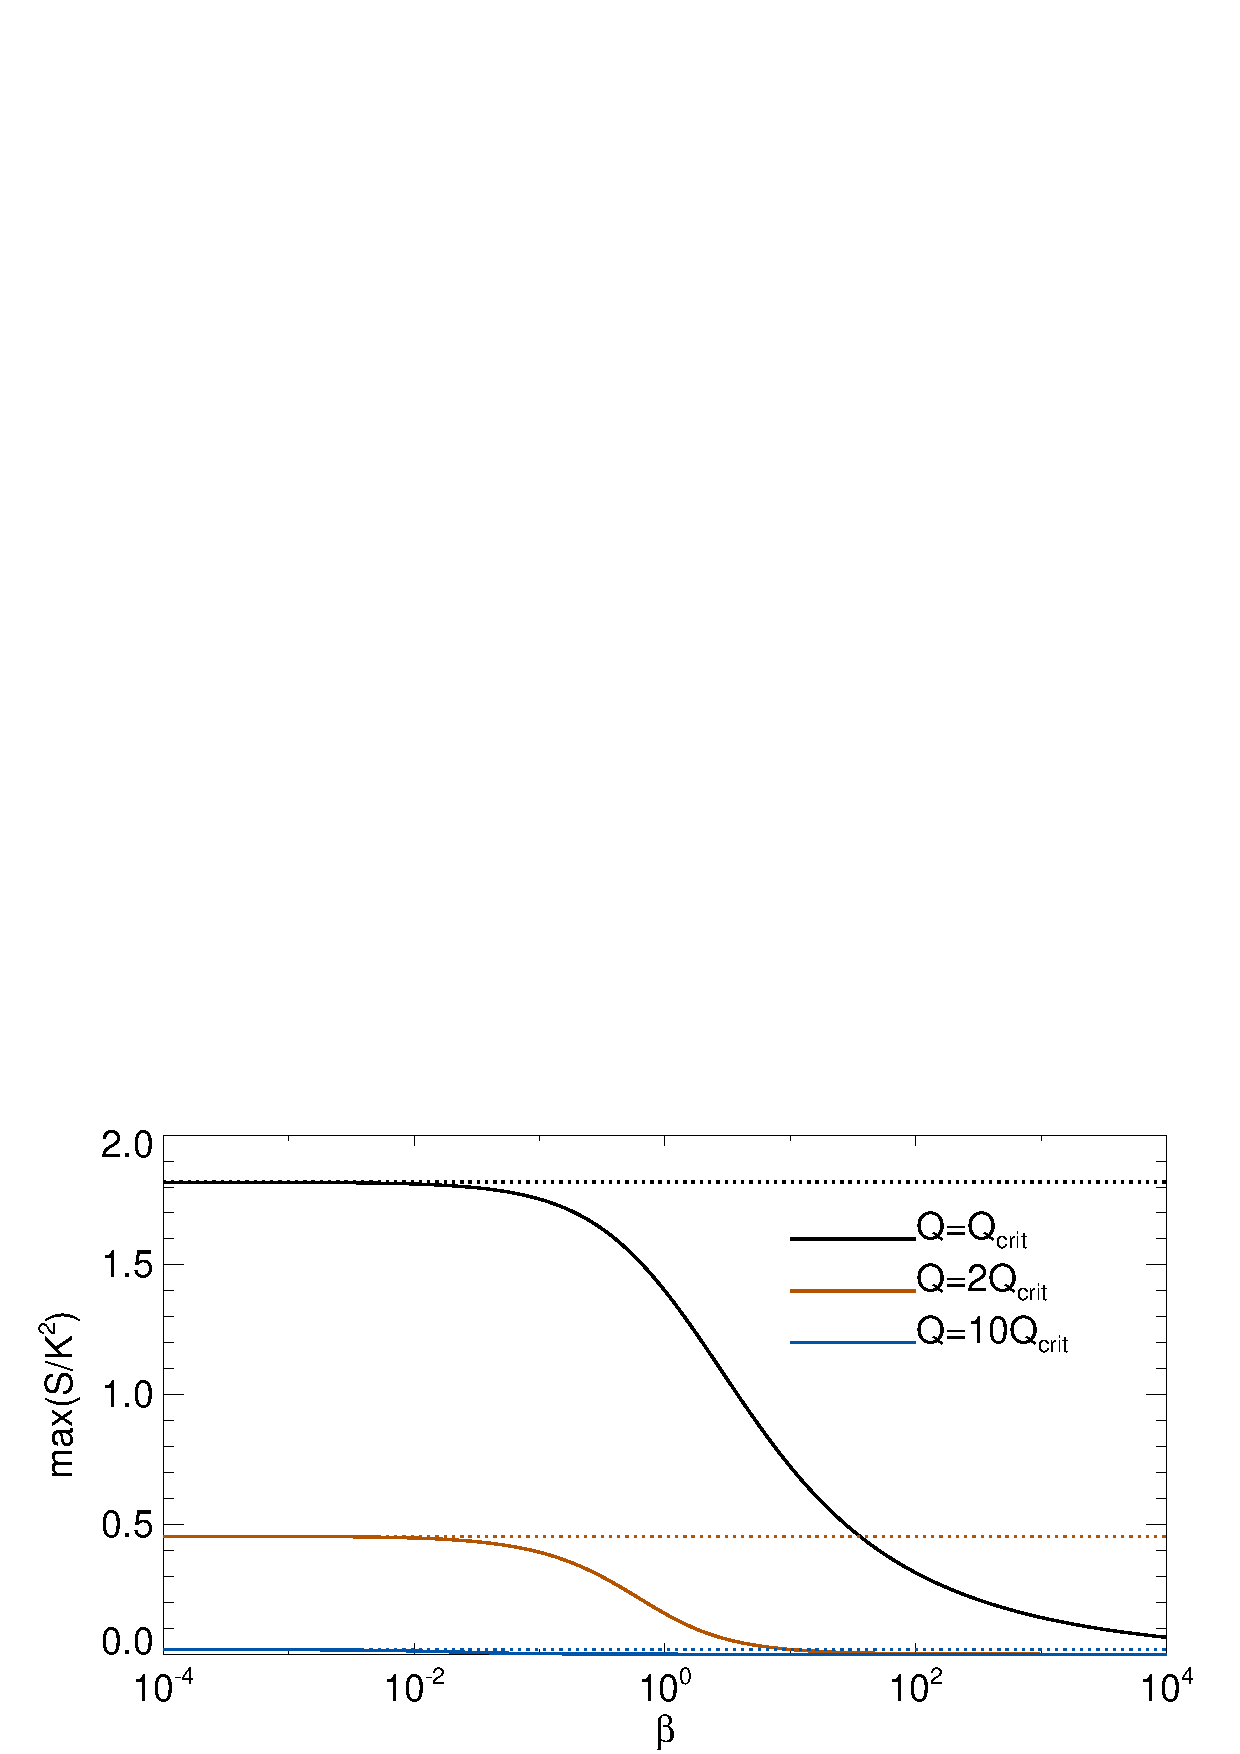
\includegraphics[width=\linewidth,clip=true,trim=0cm 0cm 0cm 0.8cm]{figures/inviscsg_alpha}
%  \caption{A measure of the
%    associated stress that can be expected in the non-linear
%    regime. The horizontal dotted lines
%    correspond to Eq. \ref{max_alpha}.}
%\end{figure}


\subsection{Viscous disk}\label{2dvisc}
We now consider a viscous disk with parameters $\mu=-1,\,\lambda=0$ in our
adopted viscosity law, Eq. \ref{visc_law}. In the 2D case this implies
$\nu\Sigma$ is constant.   
%\S\ref{visc_model}. 
We check in Appendix \ref{gammie_check} that our dispersion relation
reduces to previous results for viscous GI in the isothermal limit (by
taking $|\beta S|\to~\infty$ and $\gamma=1$).   

It is useful to consider several limiting cases.
To see the effect of cooling and irradiation, we simplify the
dispersion relation, Eq. \ref{thindisk}, by assuming $|\beta S|\ll
1$. Then for $|K| \to 0$ we find
\begin{align}\label{gammie_smallk}
%  S \sim \frac{\alpha |K|^3}{(2-q)Q},%derived assuming |beta*S|<<1 
%  S \sim \frac{\alpha K^2\left[2|K|Q^{-1} - \gamma K^2 + 2\alpha q
%    (2-q)(\gamma-1)K^2\right]}{2(2-q)+\gamma K^2 - 2|K|Q^{-1}} %derived
                                %assuming |\beta S|>>1
  S\simeq \frac{\alpha K^2}{2(2-q)}\left(\frac{2|K|}{Q} - \theta
  K^2\right), 
\end{align}
which coincides with \citeauthor{gammie96}'s Eq. 18 for vanishing
wavenumber. For $|K|\to\infty$ we find
\begin{align}\label{gammie_bigk}
  %  S \sim \frac{2}{Q|K|}\left(\frac{4}{3}\alpha + \gamma\beta\right)^{-1}.
  S \simeq\left(\frac{2}{Q|K|} - \theta\right)\left(\frac{4}{3}\alpha + 
  \alpha_b + \gamma\beta\right)^{-1}.
\end{align}

For $\theta\ll1$ a rough measure of the maximum growth rate can be obtained by
equating Eq. \ref{gammie_smallk} and \ref{gammie_bigk}\footnote{If
  $\theta$ is not small and/or $Q$  is large then one may just use Eq. \ref{gammie_smallk}
  to maximize $S$ over $K$, see the $\theta=0.3,\beta=100$ curve in the bottom
  panel of Fig. \ref{gammie_rate_plot}}.  
This exercise yields 
\begin{align}\label{gammie_maxrate_simple}
  %S_* \simeq
  %\frac{1}{Q}\left(\frac{\alpha}{2-q}\right)^{1/4}\left(\frac{6}{4\alpha
%+ 3\gamma\beta}\right)^{3/4}. 
  S_*\simeq \frac{
    6^{3/4}\left[\alpha\left(4\alpha +
      3\alpha_b + 3\gamma\beta\right)\right]^{1/4} - 3\theta
    Q(2-q)^{1/4}}{Q\left(4\alpha + 3\alpha_b +
    3\gamma\beta\right)(2-q)^{1/4}}. 
\end{align} 
%gravito-viscous instability 


%KMK moved fig ref. 
To compute growth rates numerically, 
we consider a model with $\gamma=1.4$, $\alpha_b=0$ and 
$\alpha=\alpha(\beta)$ given by thermal equilibrium
(Eq. \ref{alpha_beta_relation}). Furthermore, we relate   
\begin{align}
  Q = \frac{Q_\mathrm{crit}}{\sqrt{\alpha}},\label{Qalpha}
\end{align}
%with $Q_\mathrm{crit}$ given by 
to mimic a basic state maintained by gravito-turbulence where one
might expect the dimensionless stress $\alpha \sim Q^{-2}$
\citep{lin87}.   

%%KMK MOVED?
%As a numerical example, we consider a model with $\alpha_b=0$ and
%$\alpha=\alpha(\beta)$ given by thermal equilibrium (
%Eq. \ref{alpha_beta_relation}). Furthermore, we relate 
%\begin{align}
 % Q = \frac{Q_\mathrm{crit}}{\sqrt{\alpha}},\label{Qalpha}
%\end{align}
%%with $Q_\mathrm{crit}$ given by 
%to mimic a basic state maintained by gravito-turbulence where one
%might expect the dimensionless stress $\alpha \sim Q^{-2}$
%\citep{lin87}.   
%should really only use this Q-alpha relation for order-unity values
%of Q

%Fig. \ref{gammie_rate_plot} shows growth rates as a function of the
%wavenumber $k$ obtained from the dispersion relation
%Eq. \ref{thindisk}. 

Fig. \ref{gammie_rate_plot} shows growth rates as a function of the
wavenumber obtained from the dispersion relation 
Eq. \ref{thindisk}. The limiting behavior for small/large $K$ are
well-captured by Eq. \ref{gammie_smallk} and
\ref{gammie_bigk}. Comparing the two panels 
%of Fig. \ref{gammie_rate_plot} 
shows that increasing the
irradiation level ($\theta$) supresses small-scale
perturbations. %(This also occurs in the inviscid case.)

%The case $\beta=100$ is shown for completeness but is not physically
%consistent with gravito-turbulence, as the assumed $Q(\alpha)$
%relation (Eq. \ref{Qalpha}) imply $Q\gg 1$, whereas $Q$ of order unity
%is expected for a gravito-turbulent background. Nevertheless, it
%illustrates that viscous GI is qualitatively different to classic
%GI. Here, instability can occur for high $Q$. 

\begin{figure}
  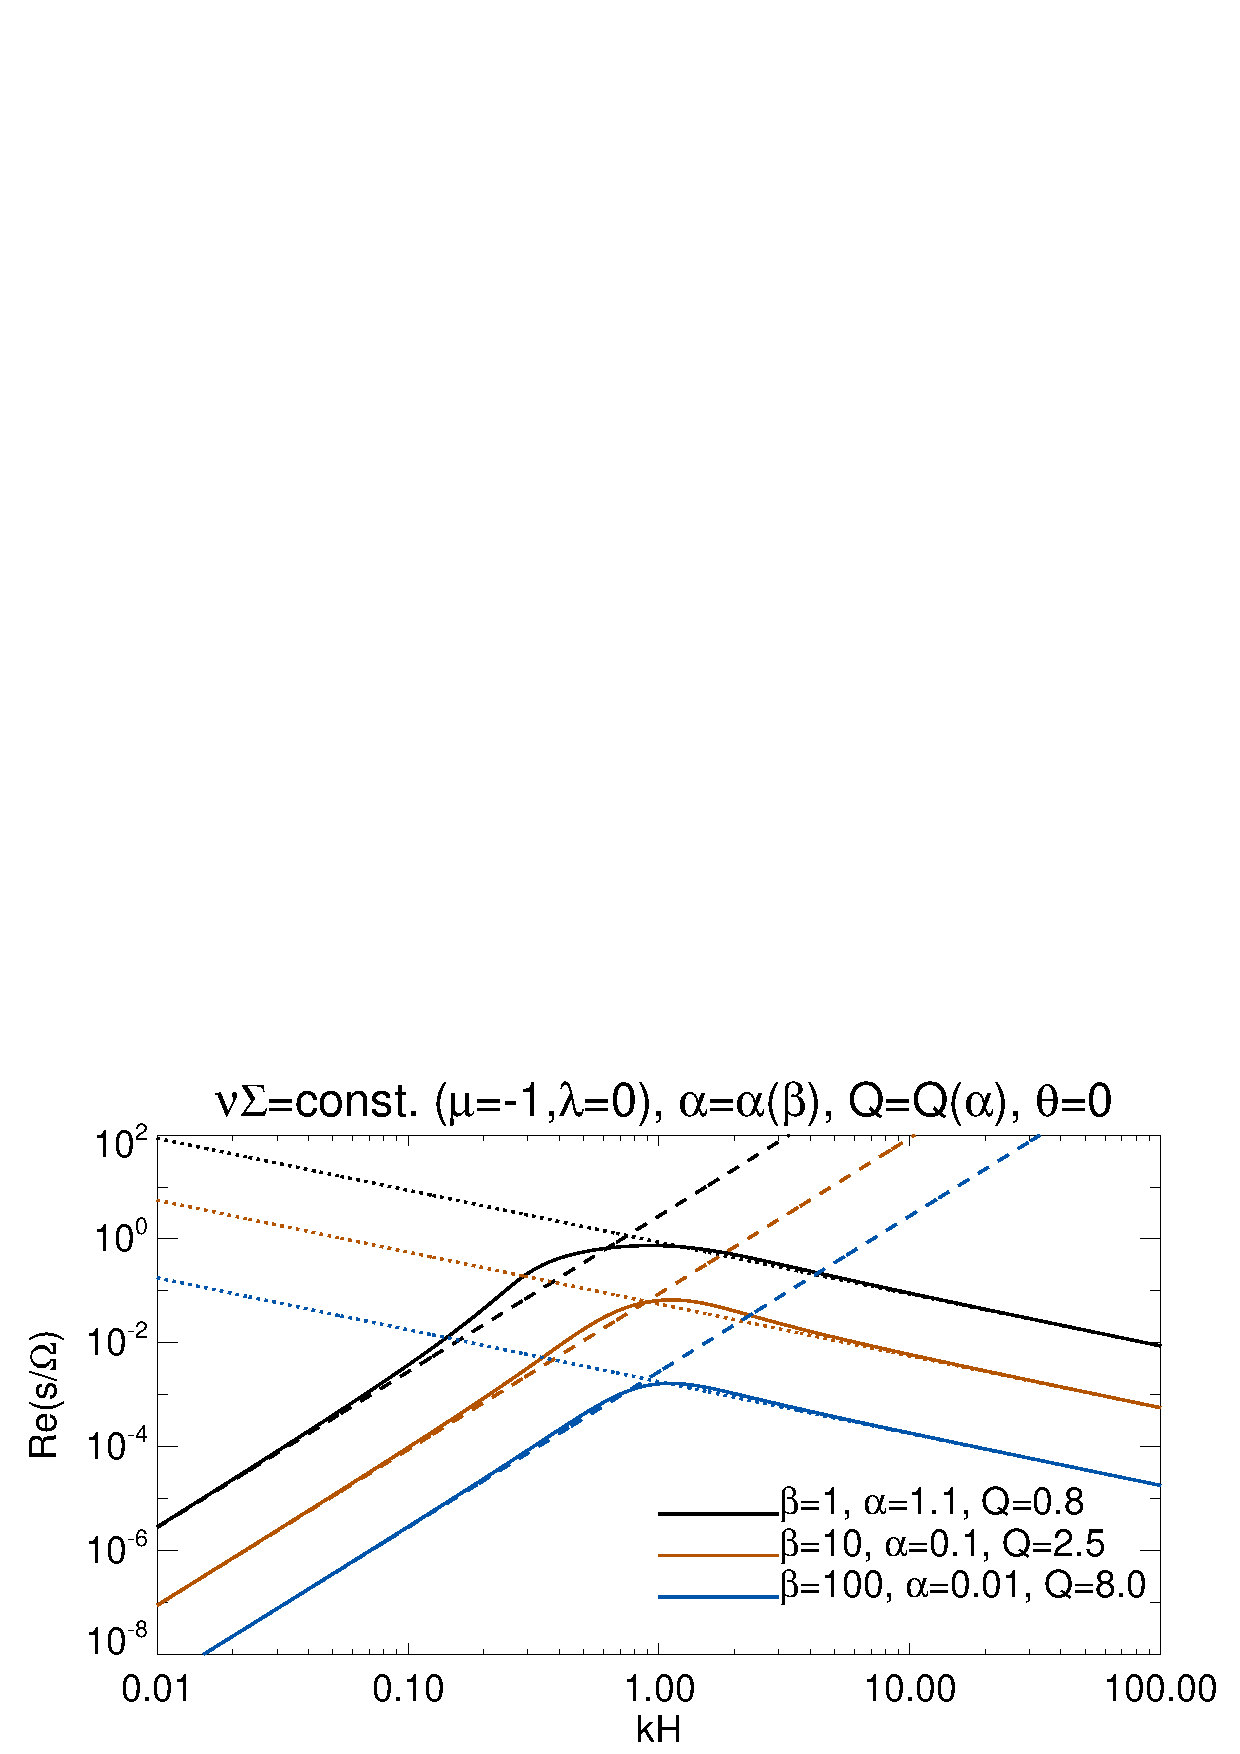
\includegraphics[width=\linewidth,clip=true,trim=0cm 2cm 0cm
    0.0cm]{figures/viscsg_modes}\\
  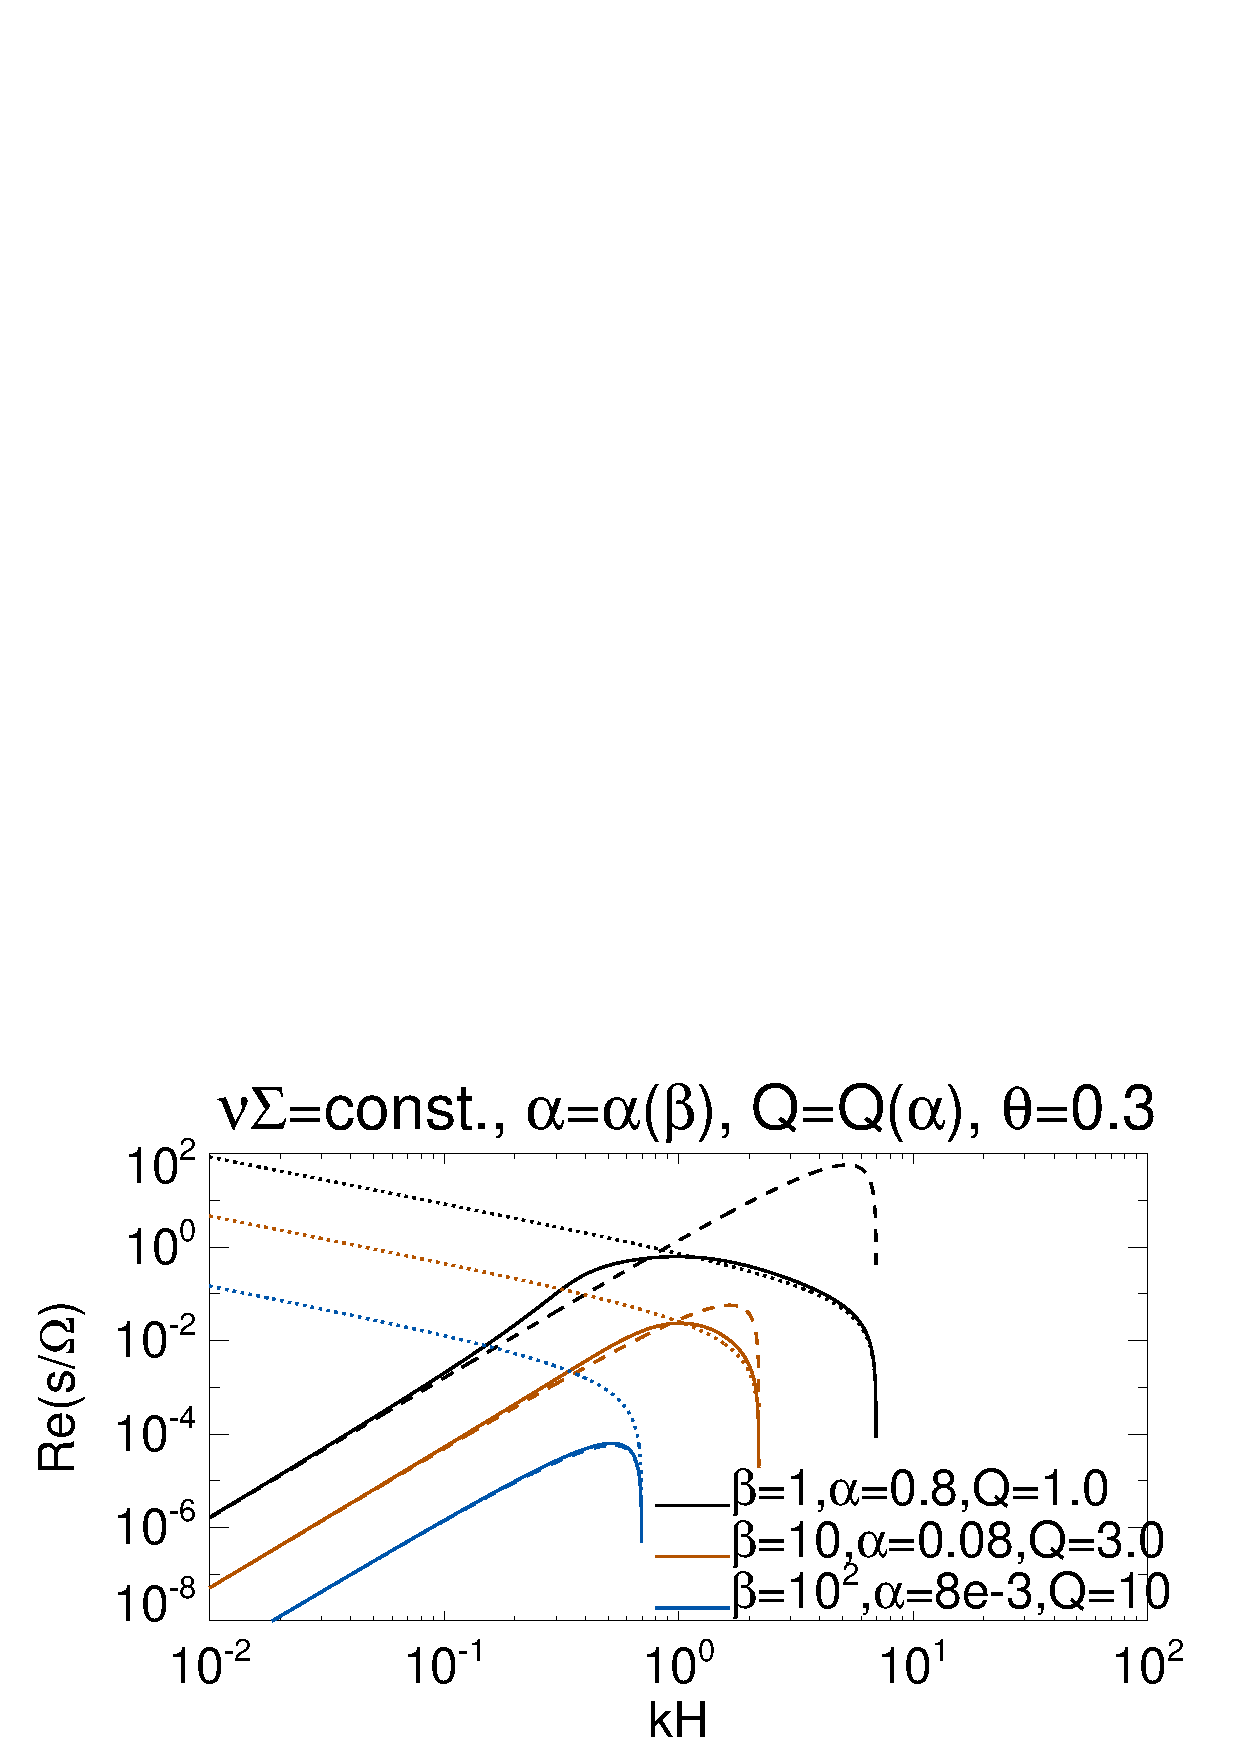
\includegraphics[width=\linewidth,clip=true,trim=0cm 0cm 0.cm
    0.0cm]{figures/viscsg_modes_theta0d3}
  \caption{Growth rates for the 2D viscous problem as a function of
    the radial wavenumber $k$ for a range of cooling times
    $\beta$. The dashed and dotted lines correspond to asympototic
    behaviors for small and large $k$, respectively, computed from
    Eq. \ref{gammie_smallk} and \ref{gammie_bigk}. Top: without
    a floor temperature ($\tirr = 0$); bottom: with a floor
    temperature $\tirr$ set to $30\%$ of the equilibrium temperature.   
    \label{gammie_rate_plot}}
\end{figure}

Fig. \ref{gammie_maxrate_plot} shows the maximum
growth rate (top panel) and the corresponding wavenumber (bottom
panel) as a function of the cooling time $\beta$ for $\theta=0$.  
There is good agreement between numerical growth rates and
Eq. \ref{gammie_maxrate_simple} for $\beta \gtrsim 1$. 
%The assumption
%of $|\beta S|\ll 1$ is not well satisfied at smaller $\beta$ which
%explains the mismatch there. 
Eq. \ref{gammie_maxrate_simple} gives the
limiting behavior for this case as   
\begin{align}
  S_*\propto \begin{cases}
%    \frac{\alpha^{1/4}}{Q\beta^{3/4}} \propto \beta^{-3/2} 
    \alpha^{1/4}\beta^{-3/4}Q^{-1}\propto \beta^{-3/2} 
    &  \beta \gg \alpha, \\
%    \frac{1}{Q\sqrt{\alpha}}  
    \alpha^{-1/2}Q^{-1} = \mathrm{const.} & \beta \ll \alpha, \label{high_visc}   
  \end{cases}
\end{align}
%{\bf KMK physically what is the limit $\beta \ll \alpha$?}
where we have applied Eq. \ref{alpha_beta_relation}
and \ref{Qalpha}. %The second limit corresponds to a hypothetical
%situation where rapid cooling is balanced by large viscous heating
%(we discuss why this). 
The disk is unstable for all $\beta$, but
growth timescales are long ($>10$ orbits) for $\beta \gtrsim
20$. %increase beta -> drop alpha -> increase Q. latter two expected
     %to stablize
This region is marked by the vertical dashed-dotted line in
Fig. \ref{gammie_maxrate_plot}. The optimum wavenumber decreases with
the cooling time for $\beta\lesssim O(1)$ because larger scales are 
more resistant to the associated increase in viscous damping. This is
evident from the dispersion relation in the large wavenumber limit,
Eq. \ref{gammie_bigk}, showing increasing viscosity weakens
small-scale modes. 
%{\bf KMK this is
%confusing b/c viscosity is in general acting on larger scales than pressure. al%so damping -> dissipation or 
%angular momentum transport?}


%{\bf maybe move following to discussion}
Numerical simulations of gravito-turbulent disks show there is a
maximum $\alpha$ ($\sim 0.06$) that can be sustained before
fragmentation \citep{rice05}. We can interpret this result in our
linear framework. 
Suppose it is possible to balance rapid cooling ($\beta\lesssim1$) 
by generating a large gravito-turbulent heating rate
($\alpha\gtrsim 1$) through a small $Q$ (second case in
Eq. \ref{high_visc}). Fig. \ref{gammie_maxrate_plot}  
shows that such a disk would be dynamically unstable with 
growth rate $s = O(\Omega)$. This is due to the direct effect of viscous 
stress promoting instability, rather than cooling. Thus, we do not expect rapidly-cooled, 
and hence highly turbulent, self-gravitating disks to persist beyond
dynamical timescales.
%KMK
We might interpret fragmentation as the response to the instability of the
highly viscous state. This is consistent with previous numerical
simulations performed by \cite{lodato05}. 
%Case (\ref{gvisc}) is consistent with 
\begin{figure}
%  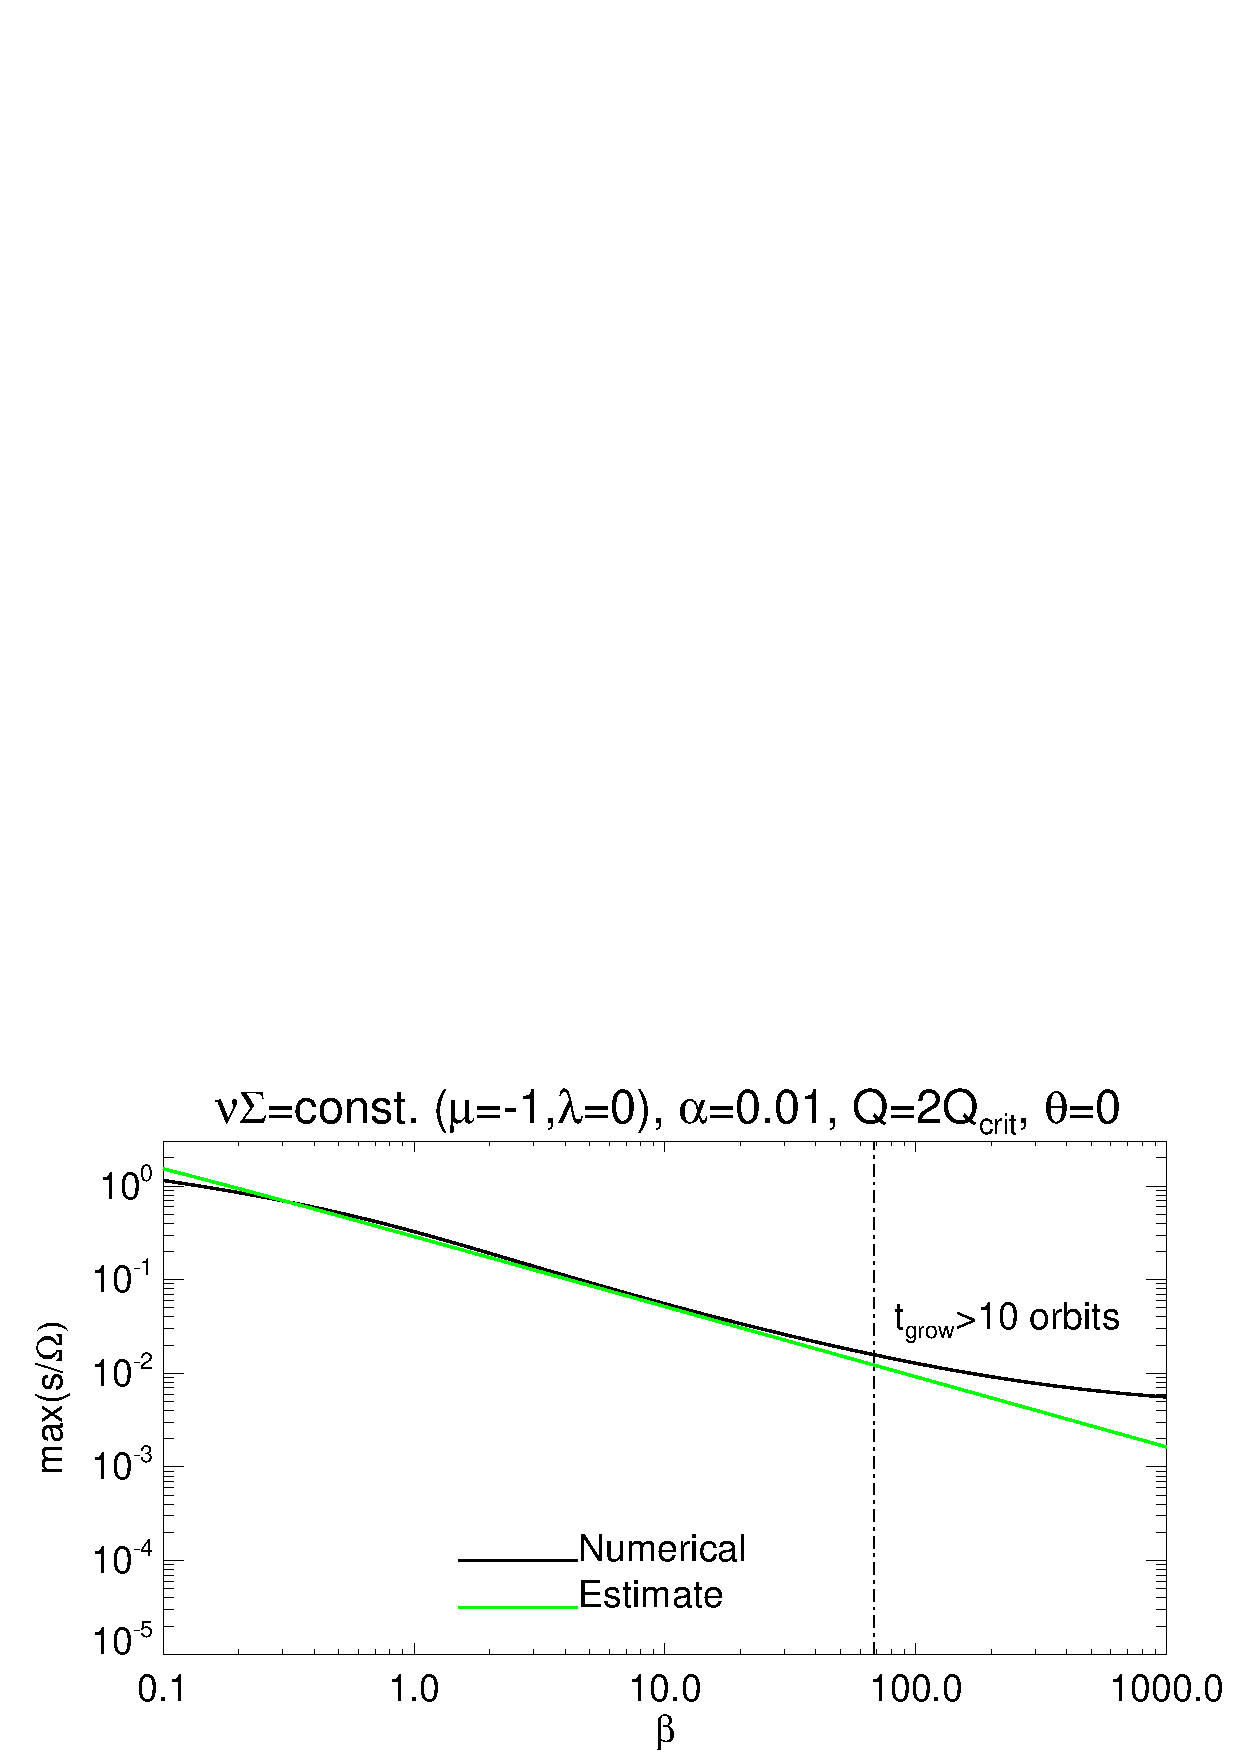
\includegraphics[width=\linewidth,clip=true,trim=0cm 1.5cm 0cm
%    0.0cm]{figures/result2d_fixalpha}\\
%  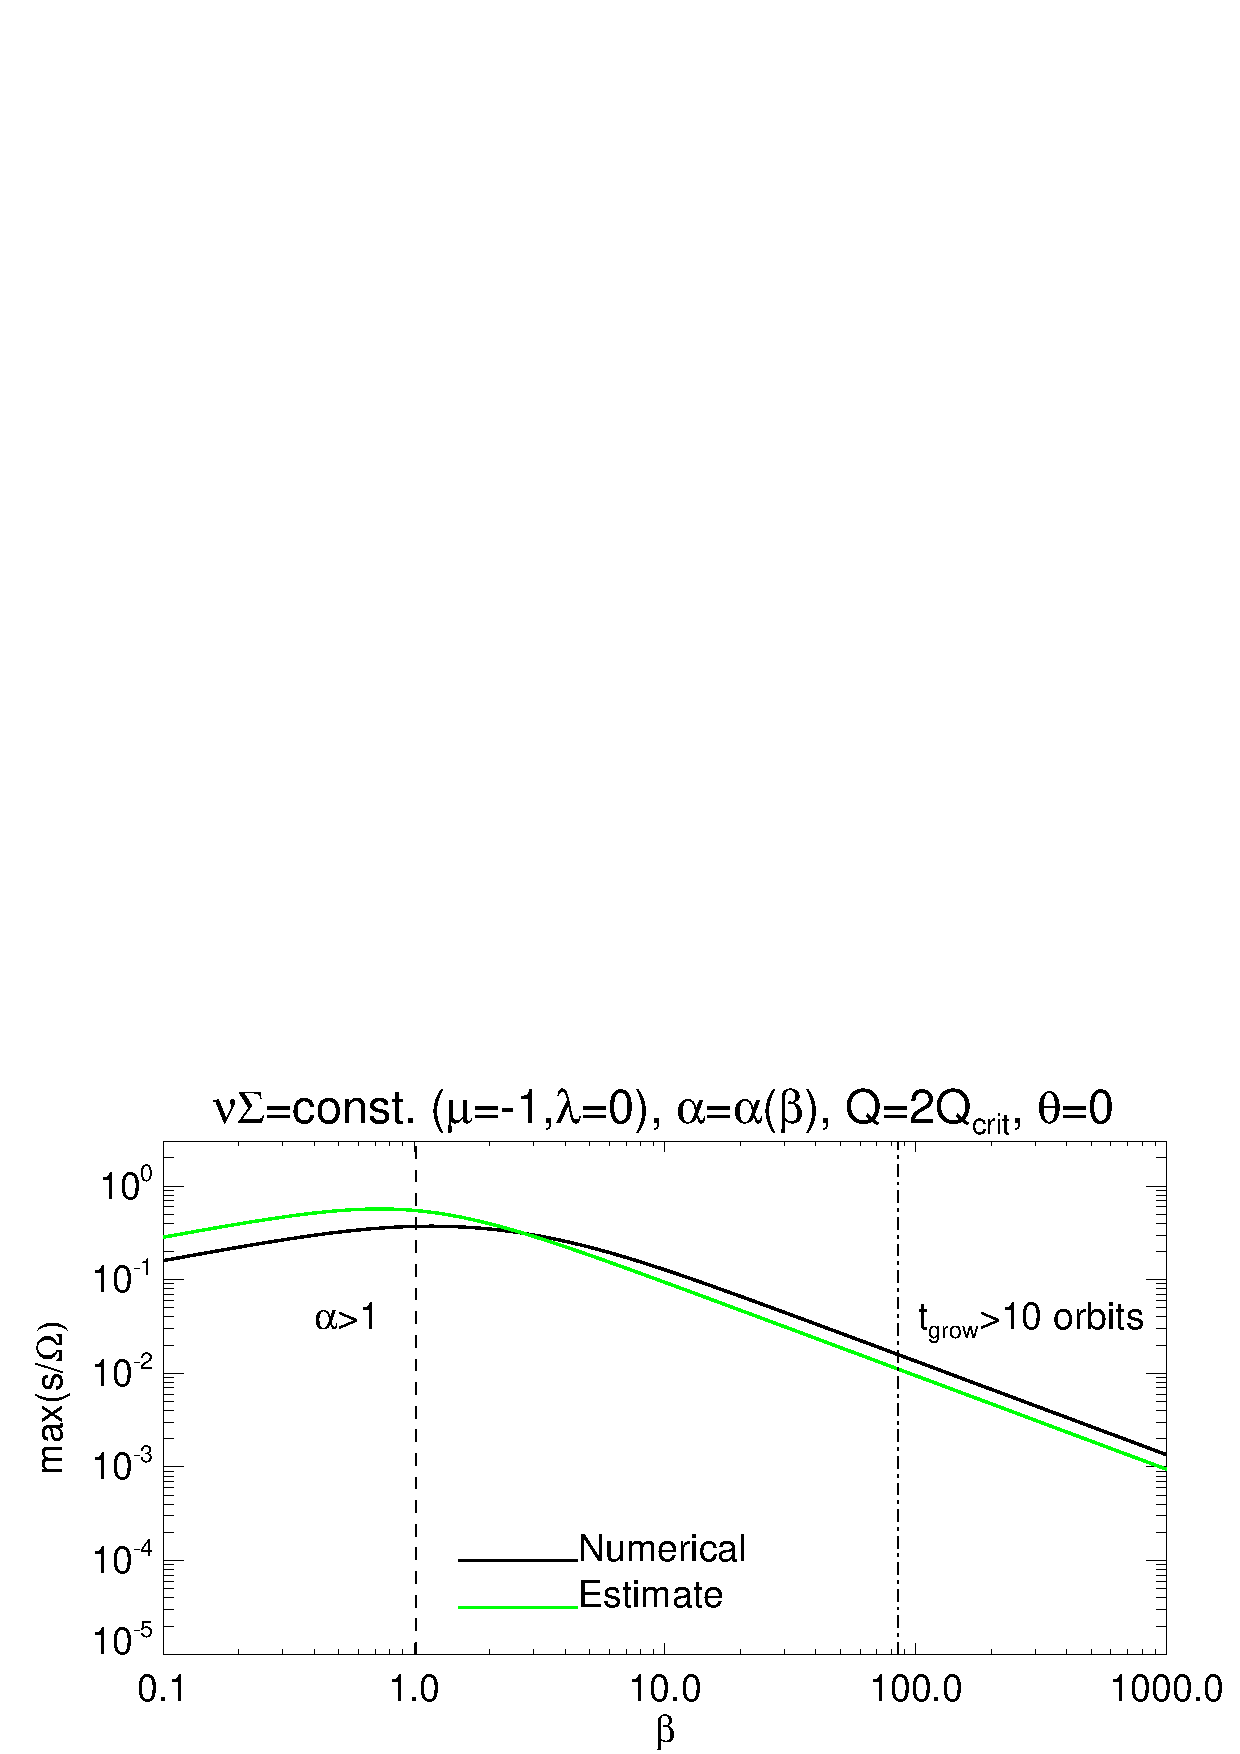
\includegraphics[width=\linewidth,clip=true,trim=0cm 1.5cm 0cm
%    0.0cm]{figures/result2d_fixQ}\\
  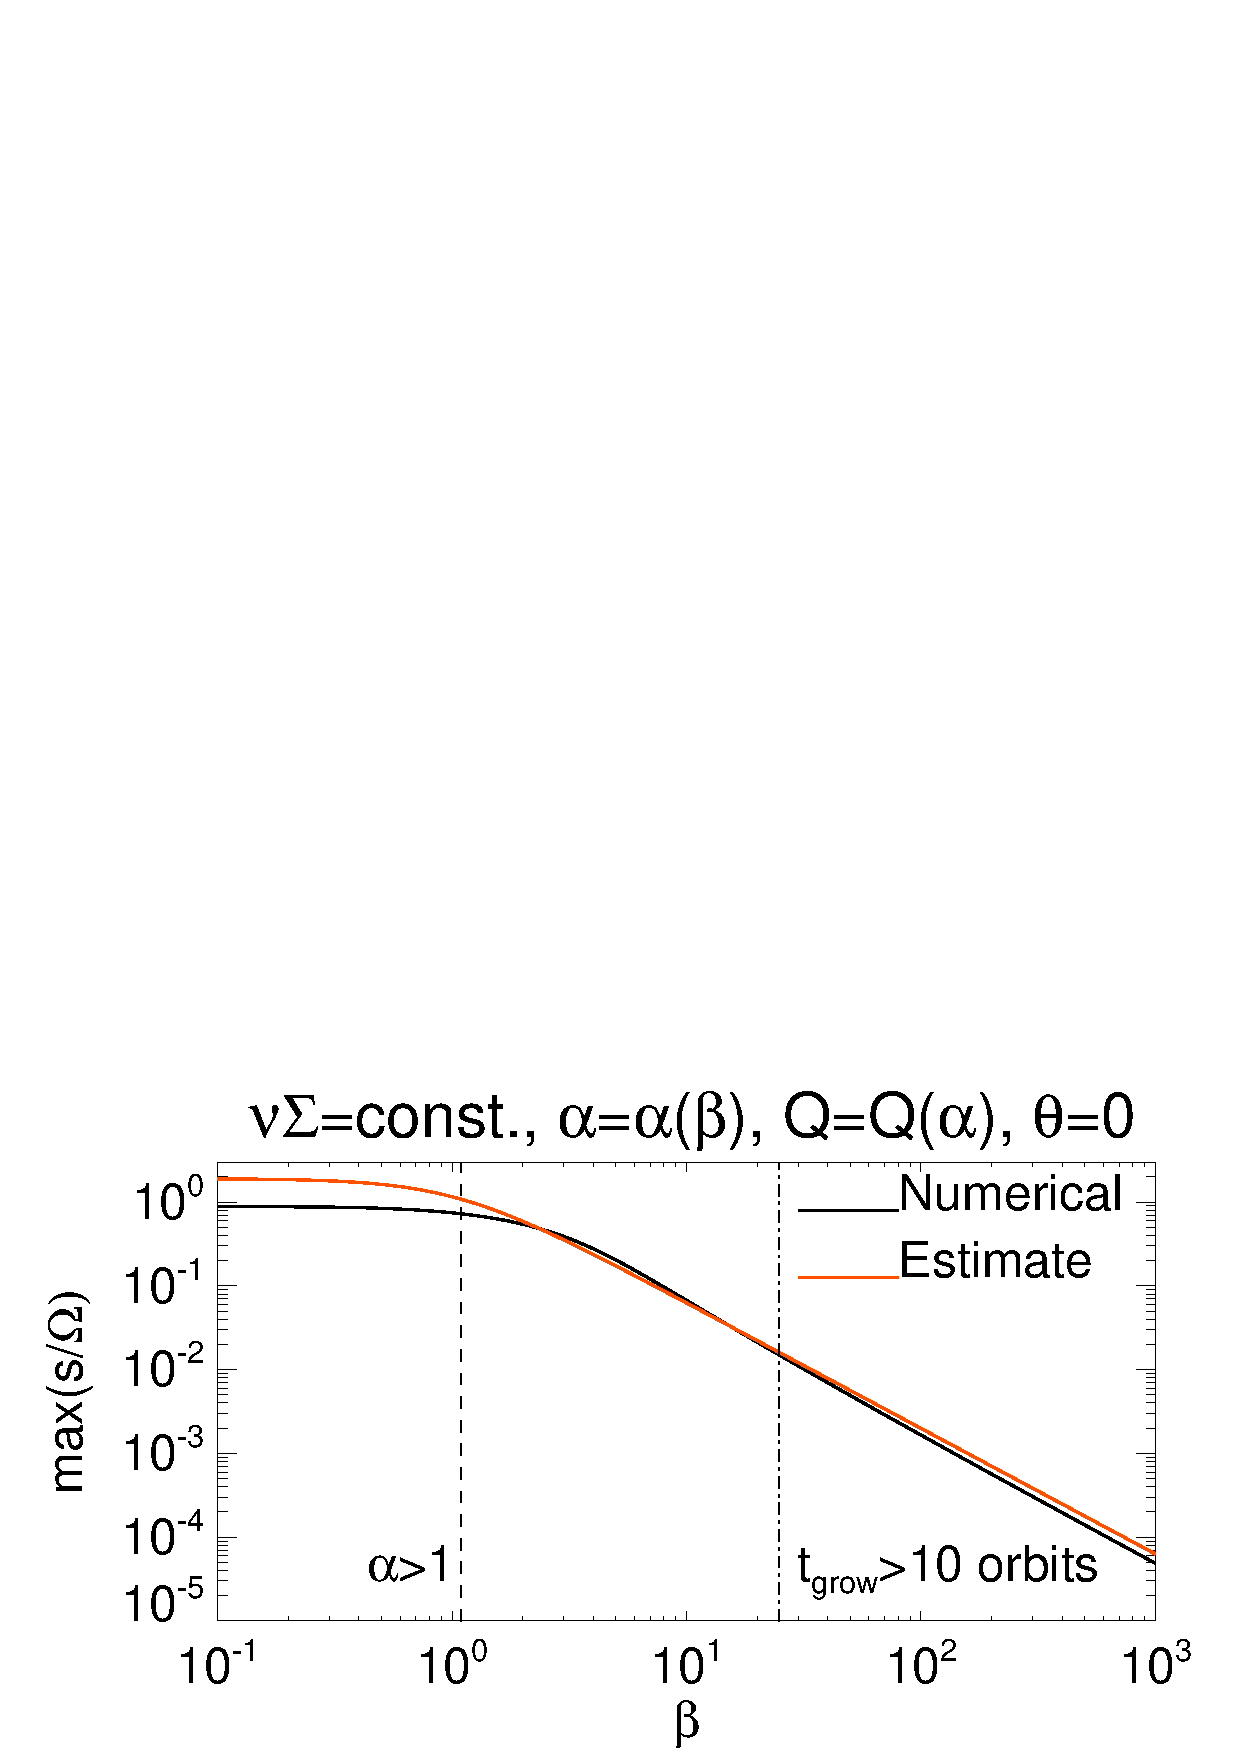
\includegraphics[width=\linewidth,clip=true,trim=0cm 2cm 0.cm
    0.0cm]{figures/result2d_gvisc}
  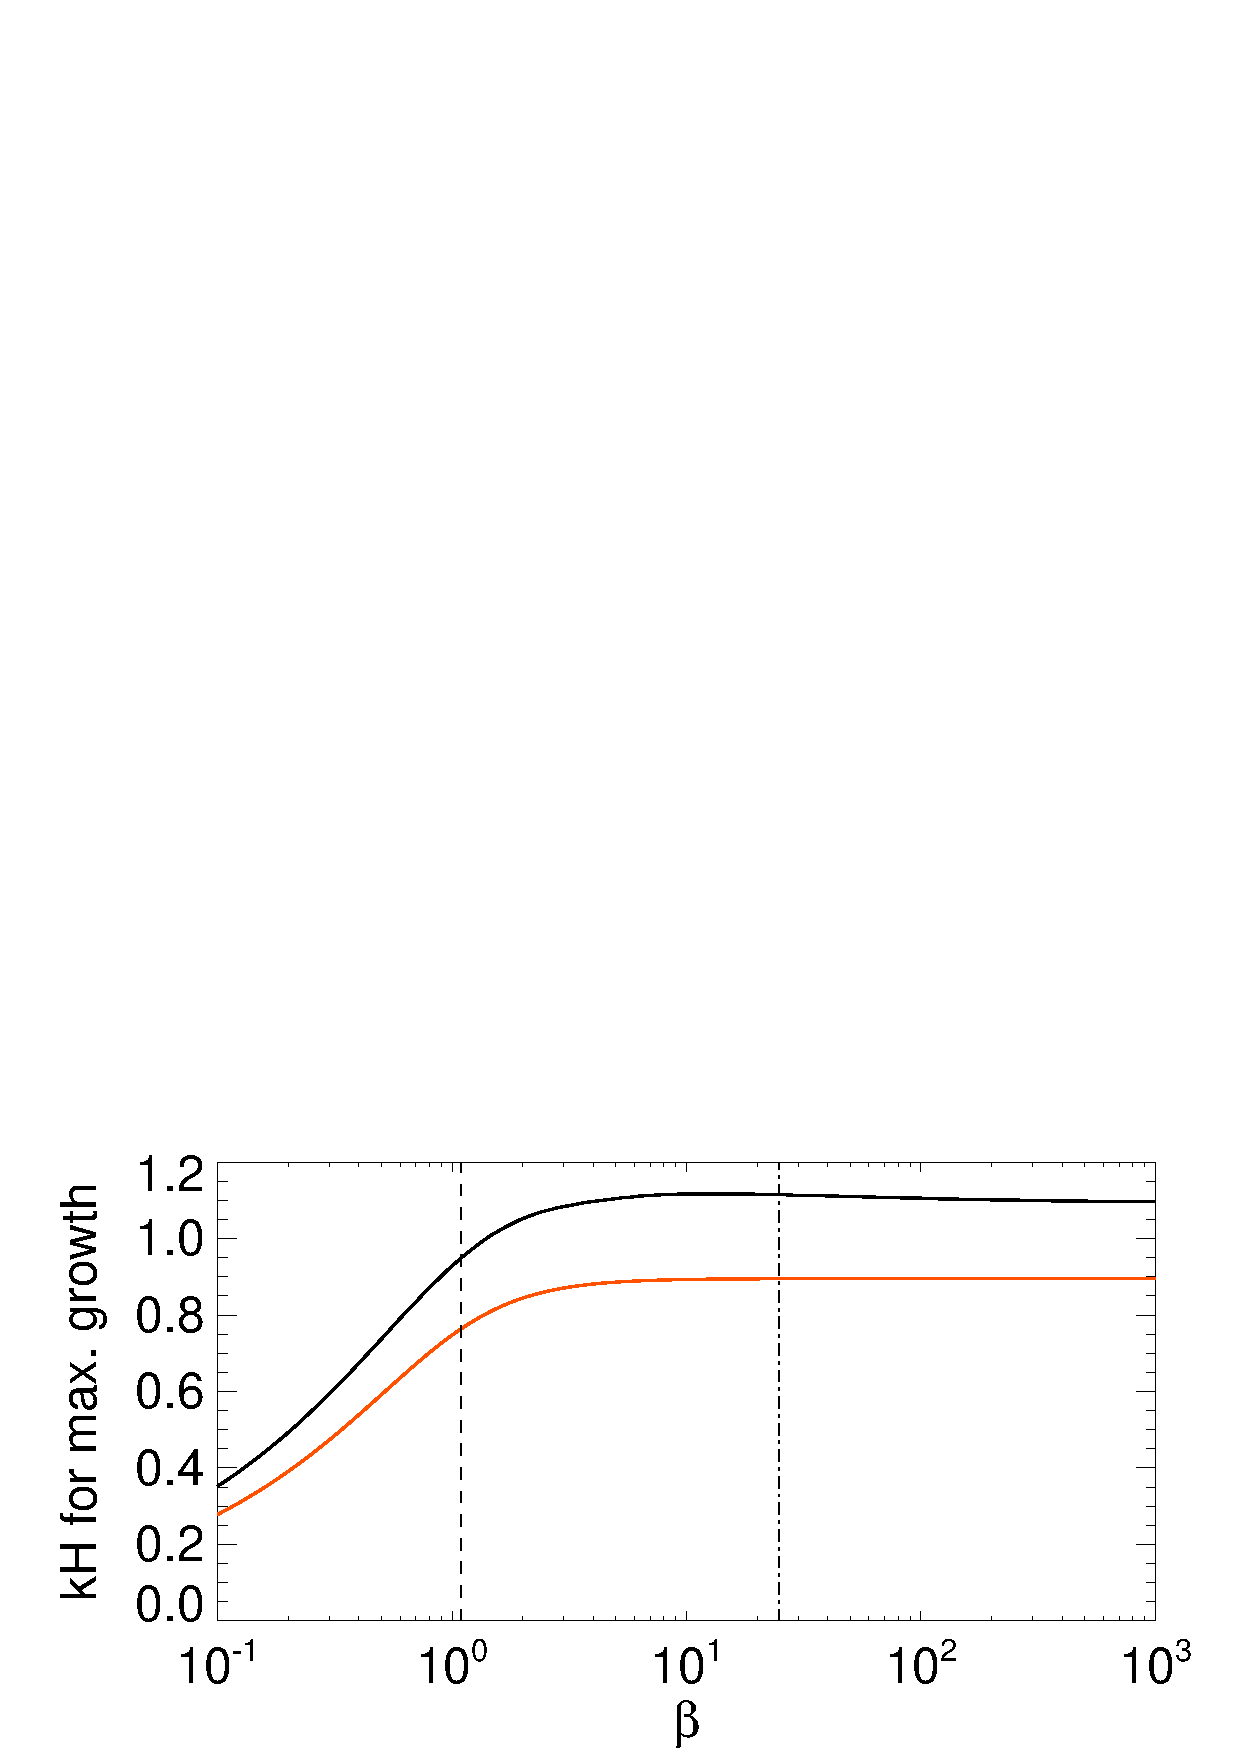
\includegraphics[width=\linewidth,clip=true,trim=0cm 0cm 0.cm
    1.0cm]{figures/result2d_gvisc_kmax}
  \caption{Growth rates (top) at the optimal wavenumber (bottom) for
    viscous GI as a function of cooling time for the
    case shown in the top panel of Fig. \ref{gammie_rate_plot}. Black curves 
    computed from the dispersion relation (Eq. \ref{thindisk}), and
    the orange curves are estimates based on
    Eq. \ref{gammie_smallk}---\ref{gammie_bigk}. 
    The dashed
    line marks the region with $\alpha > 1$, and the 
    dashed-dot line marks the region where growth timescales exceed
    the dynamical time.   
    \label{gammie_maxrate_plot}}
\end{figure}
